\chapter{Systematic Uncertainties}\label{section:star_systematics}
Apart from the statistical uncertainties there are also systematic uncertainties originating from inefficiencies and limitations of the measurement devices and techniques. 
Systematic uncertainties are obtained by using modified input distributions and calculating the difference between standard and changed settings for each bin of the distribution. The systematic uncertainties on $1/N$~$dN/dn_\textrm{ch}$ are propagated by randomly removing and adding tracks in the $n_\textrm{sel}$ distribution before  unfolding procedure.

The following sources of systematic uncertainties were considered:
\begin{itemize}
	\item the effect of off-time pile-up on TPC track reconstruction efficiency~\cite{supplementaryNote},
	\item the uncertainty of TPC track reconstruction efficiency related to the~description of dead-material in simulation~\cite{supplementaryNote},
	\item representation of data sample in embedding MC~\cite{supplementaryNote},
	\item fake track background contribution (Sec.~\ref{section:star_background_primary}),
	\item TOF system simulation accuracy~\cite{supplementaryNote},
	\item accidental background contribution (Sec.~\ref{section:star_accidentals}),
	\item the effect of alternative model of hadronisation on BBC-small efficiency (Sec.~\ref{section:star_bbc}),
	\item non-SD background contribution (Sec.~\ref{section:star_nonSD}),
	\item non-closure (Sec~\ref{section:star_closure}),%: full correction procedure was applied to the MC detector-level distributions. The difference between true-level and corrected distributions was taken as a systematic uncertainties. Due to the method of factorization of the~global efficiency into the product of single-particle efficiencies, a level of non-closure below $5\%$ is typically considered to be sufficient for the validation of the procedure.
	\item non-closure of $N_\textrm{ev}$, applied only to $p_\textrm{T}$ and $\bar{\eta}$ distributions,
	\item the $1/N_\textrm{ev}$~$dN/d\bar{\eta}$ distribution was calculated separately for events in which forward proton is on one and the other side of the IP (east-west).
\end{itemize}



\Cref{fig:results_star_nch_syst,fig:results_star_pt_syst,fig:results_star_eta_syst} show the components contributing to the total systematic uncertainty for charged particle distributions without the identification. The dominant systematic uncertainty for $p_\textrm{T}$ and $n_\textrm{ch}$ distributions is related to TOF system simulation accuracy. It affects mainly low-$p_\textrm{T}$ particles, where it is about $6\%$, and large charged particle multiplicities, where it varies up to $25\%$ for $n_\textrm{ch}=8$ and $0.02 < \xi < 0.05$. In case of $\bar{\eta}$ distribution, the systematic uncertainty on TOF mainly refers to charged particles produced at the edge of the fiducial region, for which it is about $2\%$.  However, the largest (up to $6\%$) systematic uncertainty for $\bar{\eta}$,  is related to the observed diffrence  in the distributions calculated separately with respect to the forward proton direction. The rest of the components have smaller contributions to the total systematic uncertainty. The systematic uncertainty on non-closure is at the level of $2\%$ which proves  the accuracy of the correction procedure. 



\Cref{fig:results_star_syst_pi,fig:results_star_syst_K,fig:results_star_syst_p,fig:results_star_syst_xi_part} show breakdown of all different systematics for the antiparticle-to-particle multiplicity ratio distributions. An additional systematic contribution for $\bar{p}/p$ multiplicity ratio due to proton background estimation was introduced.
Since most of the corrections are the same for particle and its antiparticle, nearly all systematic uncertainties cancel out in the antiparticle-to-particle ratios. 
The largest sources of systematics, which  do not, are related to proton background estimation and dead-material effect on TPC track reconstruction efficiency.  The former was found to be up to $5\%$, whereas the latter varies up to $2\%$ for low-$p_\textrm{T}$ $\bar{p}/p$ multiplicity ratio. 

%\clearpage
\begin{figure}[h!]
	\centering
	\thisfloatpagestyle{empty}
	\vspace{-2.5cm}
	\begin{subfigure}{.49\textwidth}
		\includegraphics[width=\textwidth,page=6]{chapters/chrgSTAR/img/syst/outSD.pdf}
	\end{subfigure}
	\begin{subfigure}{.49\textwidth}
		\includegraphics[width=\textwidth,page=13]{chapters/chrgSTAR/img/syst/outSD.pdf}
	\end{subfigure}
	\begin{subfigure}{.49\textwidth}
		\includegraphics[width=\textwidth,page=20]{chapters/chrgSTAR/img/syst/outSD.pdf}
	\end{subfigure}
	\begin{subfigure}{.49\textwidth}
		\includegraphics[width=\textwidth,page=22]{chapters/chrgSTAR/img/syst/outSD.pdf}
	\end{subfigure}
	%
	\caption{Components of the systematic uncertainties for the charged particle multiplicity in three $\xi$ regions and for the average charged particle multiplicity. }
	\label{fig:results_star_nch_syst}
	\vspace{-1.5cm}
	%\vspace{-2cm}
\end{figure}
\begin{figure}[h!]
	\thisfloatpagestyle{empty}
	\centering
	\begin{subfigure}{.49\textwidth}	
		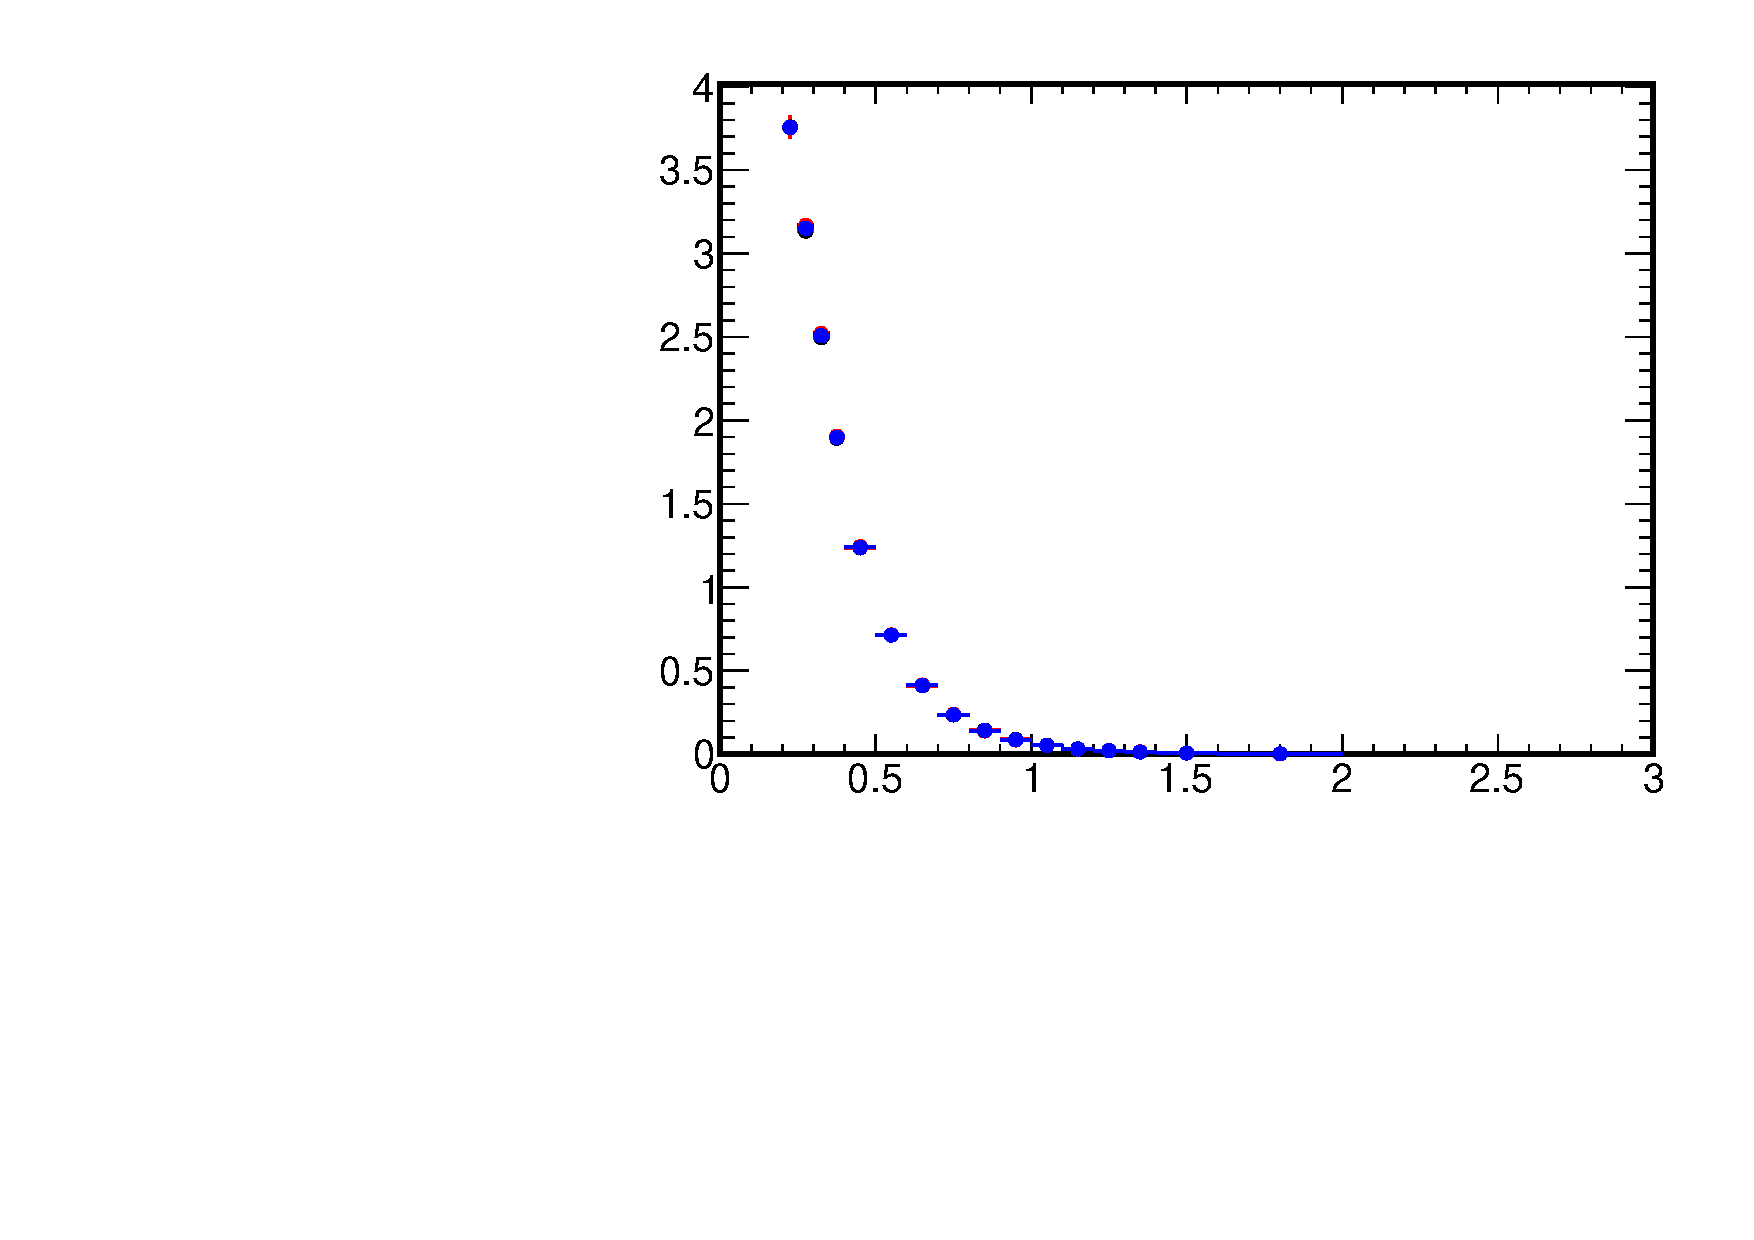
\includegraphics[width=\textwidth,page=1]{chapters/chrgSTAR/img/syst/out_chargedmax.pdf}
	\end{subfigure}
	\begin{subfigure}{.49\textwidth}
		\includegraphics[width=\textwidth,page=7]{chapters/chrgSTAR/img/syst/out_chargedmax.pdf}
	\end{subfigure}
	\begin{subfigure}{.49\textwidth}
		\includegraphics[width=\textwidth,page=13]{chapters/chrgSTAR/img/syst/out_chargedmax.pdf}
	\end{subfigure}
	\begin{subfigure}{.49\textwidth}
		\includegraphics[width=\textwidth,page=19]{chapters/chrgSTAR/img/syst/out_chargedmax.pdf}
	\end{subfigure}
	\caption{Components of the systematic uncertainties for $p_\textrm{T}$ distributions in three $\xi$ regions and for an average $p_\textrm{T}$ distribution. }
	\label{fig:results_star_pt_syst}
	%\vspace*{\floatsep}
	\vspace{-2.5cm}
\end{figure}	

\begin{figure}[h!]
	\centering
	\thisfloatpagestyle{empty}
	\vspace{-2.5cm}
	\begin{subfigure}{.49\textwidth}
		\includegraphics[width=\textwidth,page=5]{chapters/chrgSTAR/img/syst/out_chargedmax.pdf}
	\end{subfigure}
	\begin{subfigure}{.49\textwidth}
		\includegraphics[width=\textwidth,page=11]{chapters/chrgSTAR/img/syst/out_chargedmax.pdf}
	\end{subfigure}
	\begin{subfigure}{.49\textwidth}
		\includegraphics[width=\textwidth,page=17]{chapters/chrgSTAR/img/syst/out_chargedmax.pdf}
	\end{subfigure}
	\begin{subfigure}{.49\textwidth}
		\includegraphics[width=\textwidth,page=21]{chapters/chrgSTAR/img/syst/out_chargedmax.pdf}
	\end{subfigure}
	%
	\caption{Components of the systematic uncertainties for $\bar{\eta}$ distributions in three $\xi$ regions and for an average $\bar{\eta}$ distribution. }
	\label{fig:results_star_eta_syst}
\end{figure}

\begin{figure}[h!]
	\thisfloatpagestyle{empty}
	\centering
	\begin{subfigure}{.49\textwidth}
		\includegraphics[width=\textwidth,page=19]{chapters/chrgSTAR/img/syst/outPID_SDT.pdf}
	\end{subfigure}
	\begin{subfigure}{.49\textwidth}
		\includegraphics[width=\textwidth,page=20]{chapters/chrgSTAR/img/syst/outPID_SDT.pdf}
	\end{subfigure}
	\begin{subfigure}{.49\textwidth}
		\includegraphics[width=\textwidth,page=21]{chapters/chrgSTAR/img/syst/outPID_SDT.pdf}
	\end{subfigure}
	\begin{minipage}{.49\textwidth}
		\caption{Components of the systematic uncertainties of $\pi^-/\pi^+$ multiplicity ratios  in three $\xi$ regions. }
		\label{fig:results_star_syst_pi}
	\end{minipage}
	\vspace{-2.5cm}
\end{figure}


\begin{figure}[h!]
	\thisfloatpagestyle{empty}
	\vspace{-2.5cm}
	\centering
		\begin{subfigure}{.49\textwidth}
			\includegraphics[width=\textwidth,page=22]{chapters/chrgSTAR/img/syst/outPID_SDT.pdf}
		\end{subfigure}
		\begin{subfigure}{.49\textwidth}
			\includegraphics[width=\textwidth,page=23]{chapters/chrgSTAR/img/syst/outPID_SDT.pdf}
		\end{subfigure}
		\begin{subfigure}{.49\textwidth}
			\includegraphics[width=\textwidth,page=24]{chapters/chrgSTAR/img/syst/outPID_SDT.pdf}
		\end{subfigure}
		\begin{minipage}{.49\textwidth}
			\caption{Components of the systematic uncertainties of $K^-/K^+$ multiplicity ratios  in three $\xi$ regions. }
			\label{fig:results_star_syst_K}
		\end{minipage}
		
\end{figure}

\begin{figure}[h!]
	\thisfloatpagestyle{empty}
	%\vspace{-2.5cm}
	\centering
	%\vspace*{\floatsep}
	\begin{subfigure}{.49\textwidth}
		\includegraphics[width=\textwidth,page=25]{chapters/chrgSTAR/img/syst/outPID_SDT.pdf}
	\end{subfigure}
	\begin{subfigure}{.49\textwidth}
		\includegraphics[width=\textwidth,page=26]{chapters/chrgSTAR/img/syst/outPID_SDT.pdf}
	\end{subfigure}
	\begin{subfigure}{.49\textwidth}
		\includegraphics[width=\textwidth,page=27]{chapters/chrgSTAR/img/syst/outPID_SDT.pdf}
	\end{subfigure}
	\begin{minipage}{.49\textwidth}
		\caption{Components of the systematic uncertainties of $\bar{p}/p$ multiplicity ratios  in three $\xi$ regions. }
		\label{fig:results_star_syst_p}
	\end{minipage}
	\vspace{-2.5cm}
\end{figure}
\FloatBarrier
%\newpage
\begin{figure}[h!]
	%\centering
	%\vspace*{-\floatsep}
	%\vspace*{\floatsep}
	\centering
		\begin{subfigure}{.49\textwidth}
			\includegraphics[width=\textwidth,page=37]{chapters/chrgSTAR/img/syst/outPID_SDT_ratio.pdf}
		\end{subfigure}
		\begin{subfigure}{.49\textwidth}
			\includegraphics[width=\textwidth,page=38]{chapters/chrgSTAR/img/syst/outPID_SDT_ratio.pdf}
		\end{subfigure}
		\begin{subfigure}{.49\textwidth}
			\includegraphics[width=\textwidth,page=39]{chapters/chrgSTAR/img/syst/outPID_SDT_ratio.pdf}
		\end{subfigure}
		\begin{minipage}{.49\textwidth}
			\caption{Components of the systematic uncertainties of average antiparticle-to-particle multiplicity ratios  in three $\xi$ regions. }
			\label{fig:results_star_syst_xi_part}
		\end{minipage}
		%\vspace{-2.5cm}
\end{figure}

